\documentclass[tikz, convert={outext=.svg,pdf2svg}]{standalone}

\usepackage{tikz,amsmath, amssymb,bm,color}
\usetikzlibrary{shapes,arrows}
\usetikzlibrary{calc}

\definecolor{myblue}{RGB}{175, 204, 233}
\usetikzlibrary{decorations.pathreplacing}

\begin{document}
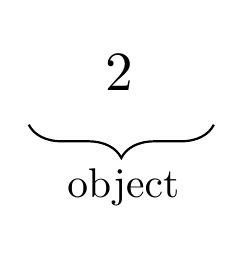
\begin{tikzpicture}

\tikzstyle{square} = [draw=none,outer sep=7,inner sep=3,minimum size=10,line width=0]
\tikzstyle{white-b} = [draw,outer sep=7,inner sep=7,minimum size=20,line width=1, 
very thick, draw=blue!25, top color=blue!25, bottom color=blue!25]
\tikzstyle{gray-b} = [draw,outer sep=7,inner sep=7,minimum size=20,line width=1, 
very thick, draw=black!100, top color=myblue, bottom color=myblue]
\tikzstyle{black_block} = [draw, text=white, font=\bf
, outer sep=7,inner sep=5,minimum size=20,line width=1,
very thick, draw=black!5, top color=black!50,bottom color=black]
\tikzstyle{gray_block}= [draw,outer sep=7,inner sep=3,minimum size=20,line width=1,very thick, draw=black!95, top color=white,bottom color=blue!25];
\tikzstyle{red_block}= [draw,outer sep=7,inner sep=3,minimum size=20,line width=1,very thick, draw=red!95, top color=white,bottom color=red!25];



\node [square, anchor=center, scale=2] at (16.45,15.6) {\begin{tabular}{c} $2$\end{tabular}};

\draw[decorate,thick, decoration={brace, amplitude=12pt}] (17.65,15)--(15.3,15);
\node[anchor=center,scale=1.5] at (16.5,14.2) {\begin{tabular}{l} object\end{tabular}}; 




\end{tikzpicture}

\end{document}